% -*- latex -*-
%%%%%%%%%%%%%%%%%%%%%%%%%%%%%%%%%%%%%%%%%%%%%%%%%%%%%%%%%%%%%%%%
%%%%%%%%%%%%%%%%%%%%%%%%%%%%%%%%%%%%%%%%%%%%%%%%%%%%%%%%%%%%%%%%
%%%%
%%%% This text file is part of the source of 
%%%% `Parallel Programming in MPI and OpenMP'
%%%% by Victor Eijkhout, copyright 2022-2023
%%%%
%%%% ompcpp_course.tex : course in C++ aspects of OpenMP
%%%%
%%%%%%%%%%%%%%%%%%%%%%%%%%%%%%%%%%%%%%%%%%%%%%%%%%%%%%%%%%%%%%%%
%%%%%%%%%%%%%%%%%%%%%%%%%%%%%%%%%%%%%%%%%%%%%%%%%%%%%%%%%%%%%%%%

\documentclass[11pt,headernav]{beamer}

\beamertemplatenavigationsymbolsempty
\usetheme{Madrid}%{Montpellier}
\usecolortheme{seahorse}
\setcounter{tocdepth}{1}
%% \AtBeginSection[]
%% {
%%   \begin{frame}
%%     \frametitle{Table of Contents}
%%     \tableofcontents[currentsection]
%%   \end{frame}
%% }

%Global Background must be put in preamble
%\usebackgroundtemplate{\includegraphics[width=\paperwidth,height=\paperheight]{newton.jpg}}

\setbeamertemplate{footline}{\hskip1em Eijkhout: OMP C++\hfill
  \hbox to 0in {\hss \includegraphics[scale=.1]{tacclogonew}}%
  \hbox to 0in {\hss \arabic{page}\hskip 1in}}

\usepackage{morewrites}

\usepackage{comment}
\input slides.inex
\input commonmacs
\input acromacs

\input slidemacs
\input snippetmacs

\input coursemacs

\begin{document}
\parskip=10pt plus 5pt minus 3pt

\title{Using OpenMP from C++}
\author{Victor Eijkhout}
\date{TACC training 2023}

\begin{frame}
  \titlepage
\end{frame}

\begin{frame}{Justification}
  OpenMP has the opportunity to exploit features of modern~C++
  that are not present in C.
  In this course we will explore:
  \begin{itemize}
  \item
    range-based iteration,
  \item
    differences in treatment between vectors and arrays,
    and various sophisticated reduction schemes.
  \end{itemize}

\end{frame}

%%%%%%%%%%%%%%%%
\sectionframe{Basic stuff}
%%%%%%%%%%%%%%%%

\begin{numberedframe}{Output streams in parallel}
  \input{cppnote-output-streams-in-parallel.cut}
\end{numberedframe}

\begin{numberedframe}{Parallel regions in lambdas}
  \input{cppnote-parallel-regions-in-lambdas.cut}
\end{numberedframe}

\begin{numberedframe}{Dynamic scope for class methods}
  \def\snippetoutputsize{\footnotesize}
  \input{cppnote-dynamic-scope-for-class-methods.cut}
\end{numberedframe}

\begin{numberedframe}{Privatizing class members}
  \input{cppnote-privatizing-class-members.cut}
\end{numberedframe}

\begin{numberedframe}{Vectors are copied, unlike arrays, 1}
  %% \input{cppnote-vectors-are-copied,-unlike-arrays.cut}
  C arrays: private pointer, but shared array:
  %
  \csnippetwithoutput{privatepointer}{examples/omp/c}{pointarray}
\end{numberedframe}

\begin{numberedframe}{Vectors are copied, unlike arrays, 2}
  C++ vectors: copy constructor also copies data:
  %
  \cxxsnippetwithoutput{privatevector}{examples/omp/cxx}{privvector}
\end{numberedframe}

%%%%%%%%%%%%%%%%
\sectionframe{Parallel loops}
%%%%%%%%%%%%%%%%

\begin{numberedframe}{Questions}
  \begin{enumerate}
  \item Do regular OpenMP loops look different in C++?
  \item Is there a relation between OpenMP parallel loops and iterators?
  \item OpenMP parallel loops vs parallel execution policies on algorithms.
  \end{enumerate}
\end{numberedframe}

\begin{numberedframe}{Range syntax}
  \input{cppnote-range-syntax.cut}
\end{numberedframe}

\begin{numberedframe}{General idea}
  OpenMP can parallelize any loop over a C++ construct
  that has a `random-access' iterator.
\end{numberedframe}

\begin{numberedframe}{C++ ranges header}
  \input{cppnote-c++20-ranges-header.cut}
\end{numberedframe}

\begin{numberedframe}{C++ ranges speedup}
  \input{cppnote-c++20-ranges-speedup.cut}
\end{numberedframe}

\begin{numberedframe}{Custom iterators, 0}
  Recall that
\begin{multicols}{2}
Short hand:
\begin{lstlisting}
vector<float> v;
for ( auto e : v )
   ... e ...
\end{lstlisting}
\columnbreak for:
\begin{lstlisting}
for ( vector<float>::iterator 
      e=v.begin();
      e!=v.end(); e++ )
  ... *e ...
\end{lstlisting}
\end{multicols}
If we want 
\begin{lstlisting}
for ( auto e : my_object )
    ... e ...
\end{lstlisting}
we need a sub-class for the iterator with methods such as
\lstinline{begin}, \lstinline{end},
  \lstinline|*| and \lstinline|++|.
\end{numberedframe}

\begin{numberedframe}{Custom iterators, 1}
  OpenMP can parallelize any range-based loop with a random-access iterator.
  \begin{multicols}{2}
    Class:
    \cxxverbatimsnippet{classwithiter}
    \columnbreak
    Main:
    \cxxverbatimsnippet{ompcustompar}    
  \end{multicols}
  %%  \input{cppnote-custom-iterators.cut}
\end{numberedframe}

\begin{numberedframe}{Custom iterators, 2}
  Required iterator methods:
  \cxxverbatimsnippet{omprandaccess}  
  This is a little short of a full random-access iterator;
  the difference depends on the OpenMP implementation.
\end{numberedframe}

\begin{numberedframe}{Custom iterators, exercise}
  Write the missing iterator methods.\\
  Here's something to get you started.
  \cxxverbatimsnippet{classwithiteriter}  
\end{numberedframe}

\begin{numberedframe}{Custom iterators, solution}
  \cxxverbatimsnippet{classwithitersol1}
\end{numberedframe}

\begin{numberedframe}{Custom iterators, solution}
  \cxxverbatimsnippet{classwithitersol2}
\end{numberedframe}

\begin{numberedframe}{OpenMP vs standard parallelism}
  Application: prime number marking
  (load unbalanced)

  \cxxverbatimsnippet{markprimeomp}
  \cxxverbatimsnippet{markprimecpp}

  Standard parallelism uses \ac{TBB} as backend
\end{numberedframe}

\begin{numberedframe}{Timing}
  \lstinputlisting{examples/tbb/cxx/primepolicy-scaling-ls6.runout}
\end{numberedframe}

\begin{numberedframe}{Reductions vs standard parallelism}
  Application: prime number counting
  (load unbalanced)

  \cxxverbatimsnippet{reduceprimeomp}
  \cxxverbatimsnippet{reduceprimecpp}

\end{numberedframe}

\begin{numberedframe}{Timing}
  \lstinputlisting{examples/tbb/cxx/reducepolicy-scaling-ls6.runout}
\end{numberedframe}

%%%%%%%%%%%%%%%%
\sectionframe{Reductions}
%%%%%%%%%%%%%%%%

\begin{numberedframe}{Questions}
  \begin{enumerate}
  \item Are simple reductions the same as in C?
  \item Can you reduce \lstinline{std::vector} like an array?
  \item Precisely \emph{what} can you reduce?
  \item Any interesting examples?
  \item Compare reductions to native C++ mechanisms.
  \end{enumerate}
\end{numberedframe}

\begin{numberedframe}{Scalar reductions}
  Same as in C,\\
  you can now use range syntax for the loop.
\end{numberedframe}

\begin{numberedframe}{Reductions on vectors}
  \input{cppnote-reductions-on-vectors.cut}
\end{numberedframe}

\begin{numberedframe}{Reduction on class objects}
  \footnotesize
  \input{cppnote-reduction-on-class-objects.cut}
\end{numberedframe}

\begin{numberedframe}{Reduction illustrated}
  \label{fig:omp-reduct}

  Reduction of four items on two threads, taking into account
  initial values.
  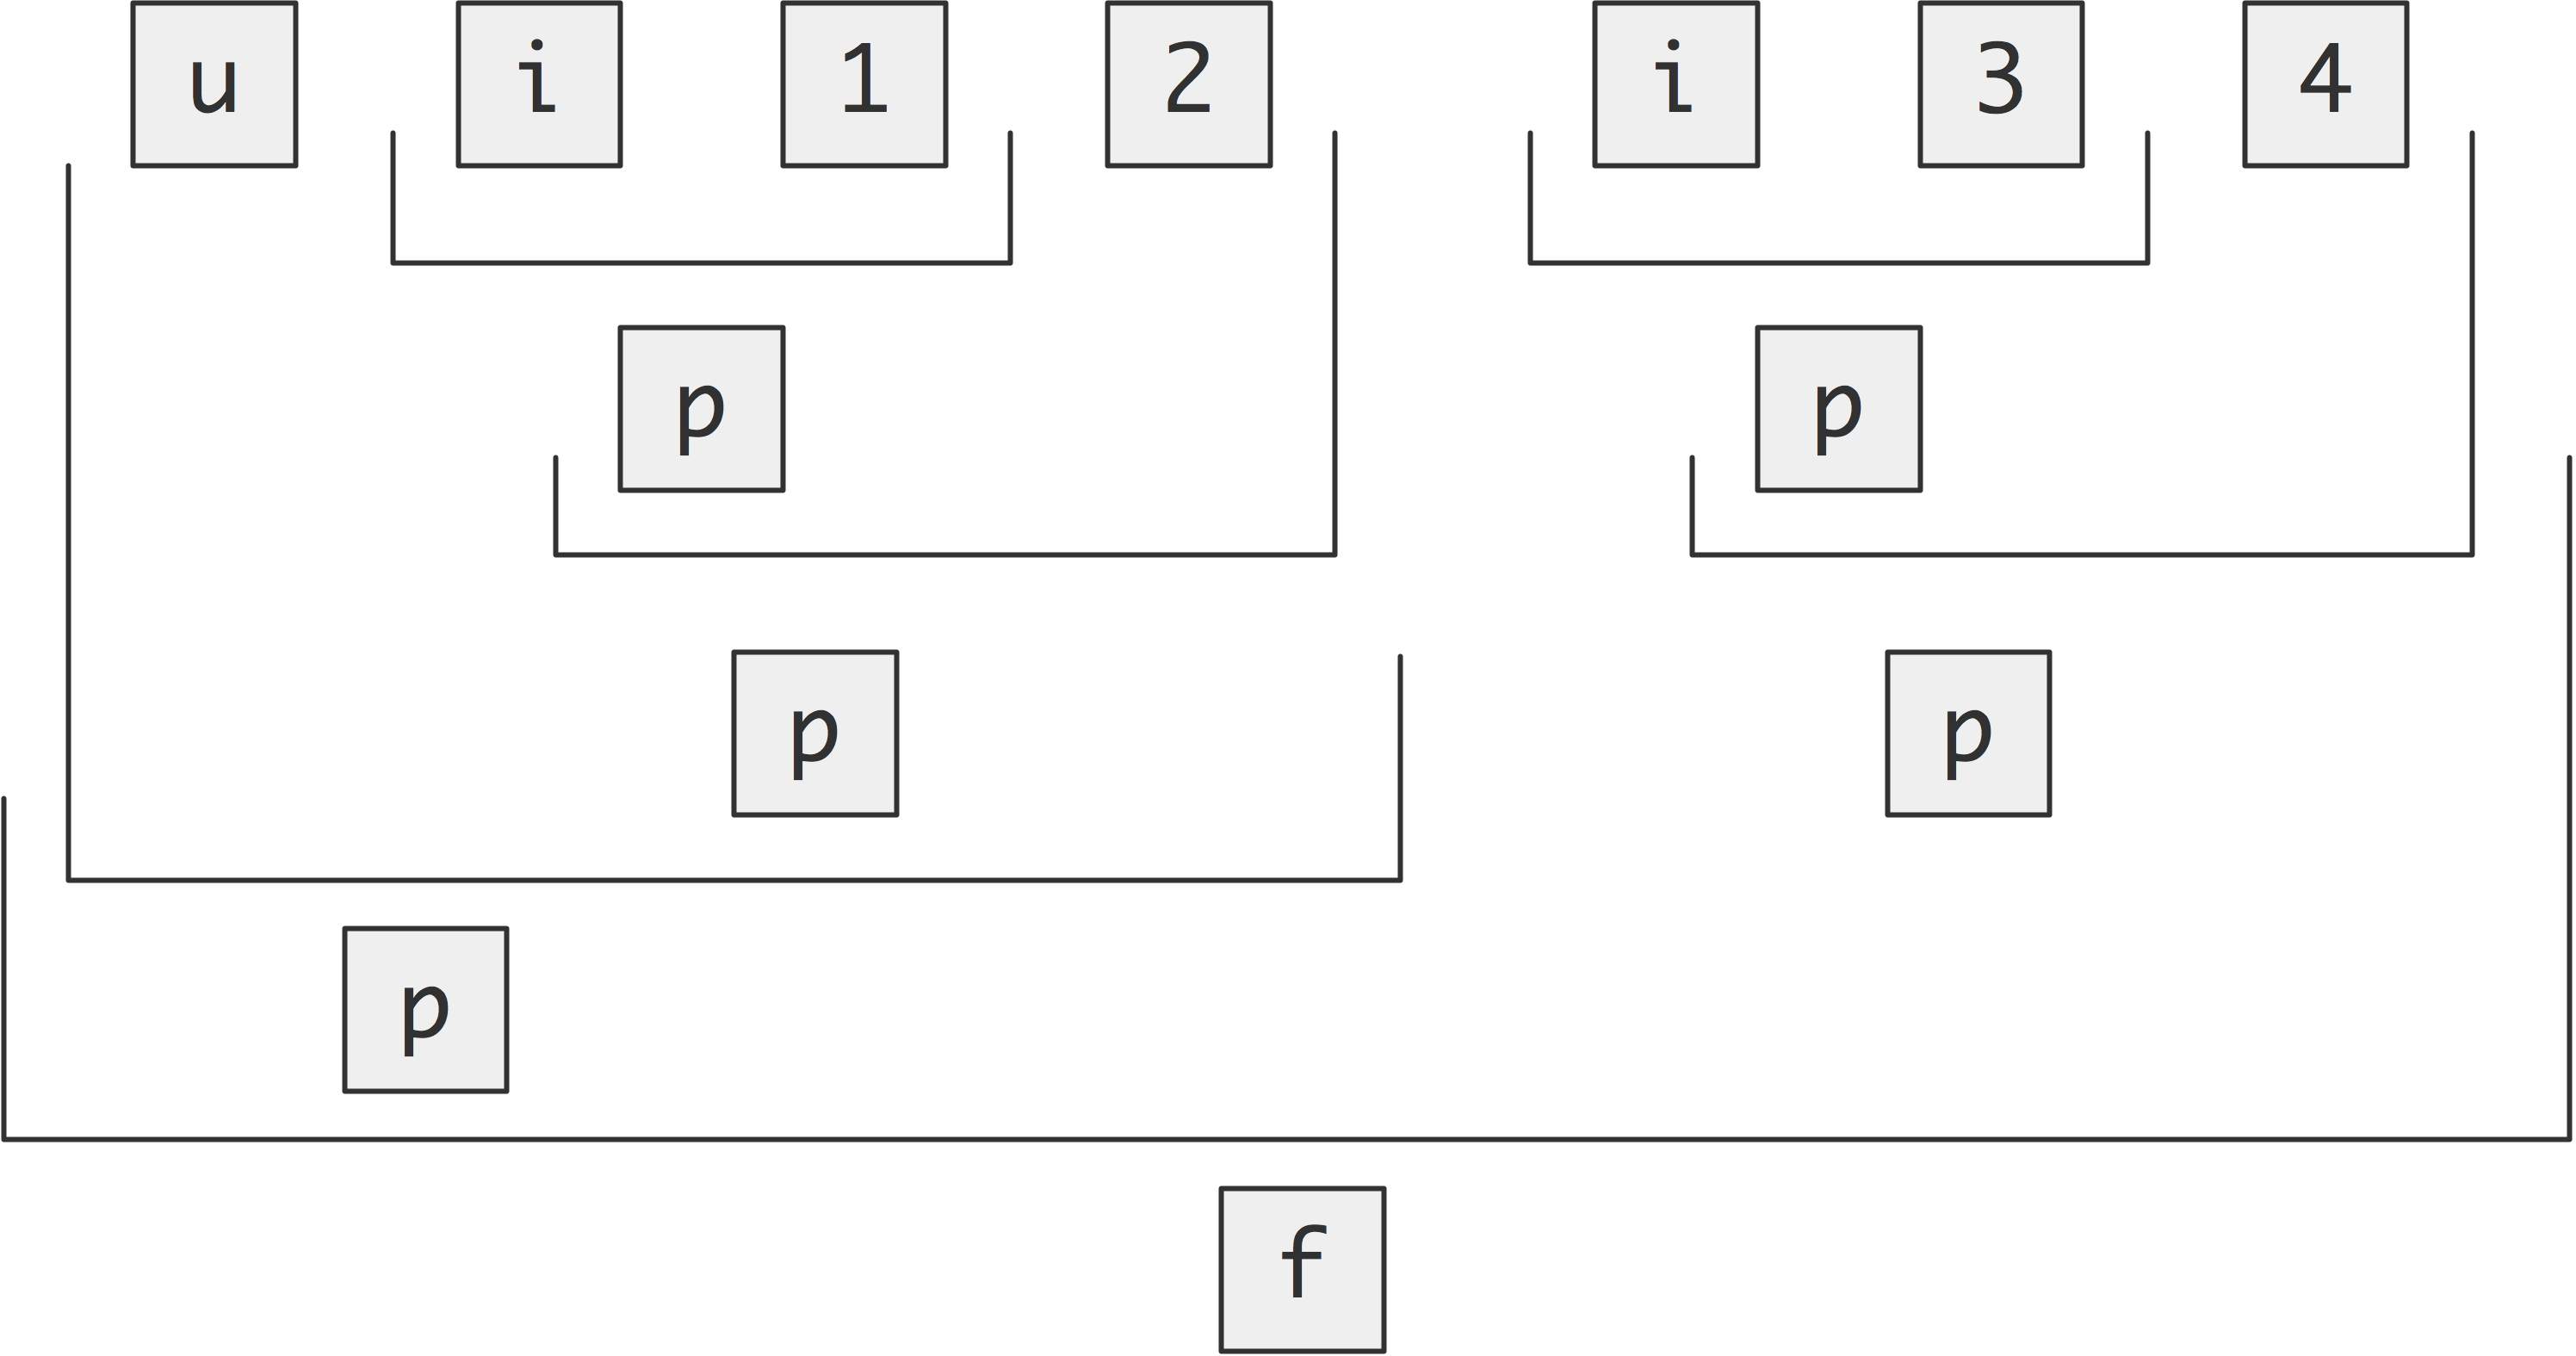
\includegraphics[scale=.1]{omp-reduct}
\end{numberedframe}

\begin{numberedframe}{User-defined reductions, syntax}
  \begin{lstlisting}
    #pragma omp declare reduction 
    ( identifier : typelist : combiner )
    [initializer(initializer-expression)]
  \end{lstlisting}
\end{numberedframe}

\begin{numberedframe}{Reduction over iterators}
  \input{cppnote-reduction-over-iterators.cut}
\end{numberedframe}

\begin{numberedframe}{Lambda expressions in declared reductions}
  \input{cppnote-lambda-expressions-in-declared-reductions.cut}
\end{numberedframe}

%% \begin{numberedframe}{Example: reduction over a map}
%%   \input{cppnote-example:-reduction-over-a-map.cut}
%% \end{numberedframe}

\begin{numberedframe}{Example category: histograms}
  Count which elements fall into what bin:
  \begin{lstlisting}
    for ( auto e : some_range )
      histogram[ value(e)]++;
  \end{lstlisting}
  Collisions are possible, but unlikely, so critical section is very inefficient
\end{numberedframe}

\begin{numberedframe}{Histogram: intended main program}
  Declare a reduction on a history gram object:
  \cxxverbatimsnippet{ompbinreduce}
  Q: why does the \lstinline{inc} not have to be atomic?
\end{numberedframe}

\begin{numberedframe}{Histogram: reduction operator}
  Give the class a \lstinline{+=} operator to do the combining:
  \footnotesize
  \cxxverbatimsnippet{ompbincounter}
\end{numberedframe}

\begin{numberedframe}{Histogram in native C++}
  Use atomics because there is no reduction mechanism:
  \cxxverbatimsnippet{atomicbincounter}
\end{numberedframe}

\begin{numberedframe}{Histogram in native C++, comparison}
  OpenMP reduction on \lstinline{array<int,26>}:
  \footnotesize
  \lstinputlisting{code/omp/cxx/mapatomic-frontera.runout}
\end{numberedframe}

\begin{numberedframe}{Example category: list filtering}
The sequential code is as follows:
\begin{lstlisting}
vector<int> data(100);
// fil the data
vector<int> filtered;
for ( auto e : data ) {
  if ( f(e) )
    filtered.push_back(e);
}
\end{lstlisting}
\end{numberedframe}

\begin{numberedframe}{List filtering, solution 1}
  Let each thread have a local array,
  and then to concatenate these:
\begin{lstlisting}
#pragma omp parallel
{
  vector<int> local;
# pragma omp for
  for ( auto e : data )
    if ( f(e) ) local.push_back(e);
  filtered += local;
}
\end{lstlisting}
where we have used an append operation on vectors:
\cxxverbatimsnippet{cppvectorplusis}
\end{numberedframe}

\begin{numberedframe}{List filtering, not quite solution 2}
We could use the plus-is operation to declare a reduction:
\cxxverbatimsnippet{cppvectorplusreduct}

Problem: OpenMP reductions can not be declared non-commutative,
so the contributions from the threads
may not appear in order.

\cxxsnippetwithoutput{cppvectordoreduct}{code/omp/cxx}{filterreduct}
\end{numberedframe}

\begin{numberedframe}{List filtering, task-based solution}
With a task it becomes possible to have a spin-wait loop:
\cxxsnippetwithoutput{cppvectordotask}{code/omp/cxx}{filtertask}
\end{numberedframe}

\begin{numberedframe}{Templated reductions}
  \input{cppnote-templated-reductions.cut}
\end{numberedframe}

%%%%%%%%%%%%%%%%
\sectionframe{More topics}
%%%%%%%%%%%%%%%%

\begin{numberedframe}{Threadprivate random number generators}
  \input{cppnote-threadprivate-random-number-generators.cut}
\end{numberedframe}

\begin{numberedframe}{Uninitialized containers}
  Multi-socket systems:\\
  parallel initialization instantiates pages on sockets:\\
  `first touch'
  \begin{lstlisting}
    double *x = (double*)malloc( N*sizeof(double));
    #pragma omp parallel for
    for (int i=0; i<N; i++)
      x[i] = f(i);
  \end{lstlisting}
  This does not work with
  \begin{lstlisting}
    std::vector<double> x(N);
    #pragma omp parallel for
    for (int i=0; i<N; i++)
      x[i] = f(i);
  \end{lstlisting}
  because of value initialization in the \lstinline{vector} container.
\end{numberedframe}

\begin{numberedframe}{Uninitialized containers, 2}
  Trick to create a vector of uninitialized data:
  %
  \cxxverbatimsnippet{cppuninitial}
  %
  so that we can create vectors that behave normally:
  %
  \cxxverbatimsnippet{cppuninitialvec}
  %% \input{cppnote-uninitialized-containers.cut}
  (Question: why not use \lstinline{reserve}?)
\end{numberedframe}

\begin{numberedframe}{Uninitialized containers, 3}
  Easy way of dealing with this:
\begin{lstlisting}
template<typename T>
class ompvector : public vector<uninitialized<T>> {
public:
  ompvector( size_t s )
    : vector<uninitialized<T>>::vector<uninitialized<T>>(s) {};
};
\end{lstlisting}
\end{numberedframe}

\begin{numberedframe}{Atomic updates}
  Pragma \lstinline{atomic} only works for simple cases.
  Can you atomically do more complicated updates?
  \begin{itemize}
  \item Make an object that has data plus a lock;
  \item Disable copy and copy-assignment operators;
  \item Destructor does \indexompshow{omp_destroy_lock};
  \item Overload arithmetic operator.
  \end{itemize}
\end{numberedframe}

\begin{numberedframe}{Atomic updates: class with OMP lock}
  \cverbatimsnippet[examples/omp/cxx/lockobject.cxx]{lockobject}
\end{numberedframe}

\begin{numberedframe}{Atomic updates: atomic ops}
  \cverbatimsnippet[examples/omp/cxx/lockobject.cxx]{lockobjectops}
\end{numberedframe}

\begin{numberedframe}{Atomic updates: usage}
  \cverbatimsnippet[examples/omp/cxx/lockobject.cxx]{lockobjectuse}
\end{numberedframe}

\begin{numberedframe}{Atomic updates, comparison to native}
  Timing comparison on simplest case:
\begin{multicols}{2}
  \lstset{basicstyle=\scriptsize}
  Object with built-in lock:
\cxxverbatimsnippet{lockobjectuse}
\columnbreak
Native C++ atomics:
\cxxverbatimsnippet{atomicintuse}
\end{multicols}

  Native solution is 10x faster.

\end{numberedframe}

\begin{numberedframe}{False sharing prevention}
  \begin{lstlisting}
    #include <new>

    #ifdef __cpp_lib_hardware_interference_size
    const int spread = std::hardware_destructive_interference_size
            / sizeof(datatype);
    #else
    const int spread = 8;
    #endif

    vector<datatype> k(nthreads*spread);
    #pragma omp parallel for schedule( static, 1 )
    for ( datatype i = 0; i < N; i++ ) {
      k[ (i%nthreads) * spread ] += 2;
  \end{lstlisting}
\end{numberedframe}

\begin{numberedframe}{Beware vector-of-bool!}
  Does not compile:
  \cxxverbatimsnippet{boolrange}
  More subtle:
  \cxxsnippetwithoutput{booliter}{code/omp/cxx}{booliter}
  Different \lstinline{bits[i]} are falsely shared.
\end{numberedframe}

\begin{numberedframe}{CMake}
  \lstinputlisting{../../makefiles/CMakeLists.omp.cxx.txt}
\end{numberedframe}

\end{document}

